\section{Theoretical Analysis}
\label{analysis}

\paragraph{}
This theoretical analysis has, as its main purpose, showing how this circuit would behave in theory. This section is divided in two given that this circuit, as explained in the theoretical introduction, is mainly composed of two different stages - the gain stage and the output stage. However, there will also be a third subsection in which we will include the frequency response analysis for the whole circuit.

The values for the multiple components of the circuit can be found below:
\[ 
\left\{\begin{matrix}
	R_{in}= 100 \Omega\\	
	R_{B1}= 80000 \Omega\\
	R_{B2}= 18000 \Omega\\
	R_E= 100\Omega\\
	R_C= 800\Omega\\
	R_{out}= 750 \Omega\\
	R_L= 8\Omega\\
	C_i=50 uF\\
	C_b=50 uF\\
	C_o=1 uF\\
	
	V_{BEON}=\approx 0.7 V\\
\end{matrix}\right.
\]

\subsection{The Gain Stage}

\paragraph{}As already explained in the very first section of this report, the final objective of this lab assignment is to make an amplifier. Given so, this stage will have, as its main goal, to get a voltage gain as high as possible. In this subsection, the OP analysis of circuit will be made (DC current) and the gain, plus the input and output impedances,  will be calculated.


\subsubsection{OP Analysis}

\paragraph{}The first subject being analyzed is how does the circuit behave when the current is continuous (DC). This part is crucial when it comes to the study of the rest of the topics, such as the impedances, given that the incremental parameters of the transistors will be calculated based on the values obtained in the OP analysis.


\[ 
\left\{\begin{matrix}
	R_{B1}= 80000 \Omega\\
	R_{B2}= 18000 \Omega\\
	R_B=\frac{R_{B1}R_{B2}}{R_{B1}+R_{B2}}\\
	V_{BEON}=\approx 0.7 V\\
	I_E=(1+\beta_F)I_B\\
	V_E=R_E I_E\\
	V_C=R_C I_C\\
	V_O=V_{CC}-V_C\\
\end{matrix}\right.
\]


\subsubsection{Voltage Gain}


\paragraph{}In order to compute the voltage gain, the values of transistor's incremental parameters are required, given by the expressions below: 

\begin{equation}
    g_m=\frac{I_C}{V_T}
\end{equation}

\begin{equation}
    r_\pi=\frac{\beta_F}{g_m}
\end{equation}

\begin{equation}
    r_o\approx\frac{V_A}{I_C}
\end{equation}


\begin{equation}
    \frac{v_o}{v_i}=-g_m(R_C||r_o)\frac{r_\pi||R_{B1}||R_{B2}}{R_S+r_\pi||R_{B1}||R_{B2}}v_S
\end{equation}

In which $v_S$ is the voltage supplied by the source. 



\subsubsection{Input and Output Impedances}

\paragraph{}Yet another very important property of this stage to be studied are the impendances, both the input and output ones. The relevance of the impedance, specially the output one, is that it gives an indication about the type of components that can be connected to it. Thus, through deductions made in the theoretical classes, the final expressions that give the required values are the following:


%\begin{equation}
%    Z_I=\frac{(r_o+R+R_E)(r_\pi+R_B+R_E)+g_m R_E r_o r_\pi-R^2_E}{r_o+R+R_E}
%\end{equation}

%\begin{equation}
%    Z_O=R_C||\frac{r_o[(R_B+r_\pi)||R_E]}{r_o||r_%\pi+ R_B||R_E\frac{r_\pi+R_B}{g_m r_\pi}}
%\end{equation}

\begin{equation}
    Z_I=R_{B1}||R_{B2}||r_\pi
\end{equation}

\begin{equation}
    Z_O=R_C||r_o
\end{equation}


\paragraph{}And so, the final results for this stage were obtained:

\begin{table}[H]
\centering
\begin{tabular}{|l|l|} 
\hline
\multicolumn{2}{|l|}{\textbf{Gain Stage Computations}}  \\ 
\hline
Data             & Values                               \\ 
\hline
        
 Voltage Gain     &  -9.598990   \\ \hline
 Input Impedance  &  32258.268036   \\ \hline
 Output Impedance &  942.142024   \\ \hline
\end{tabular}
\end{table}

\paragraph{}Analyzing the table above with detail, there are two specific values that are of great interest to this report: the voltage gain and the output impedance. When coming to the voltage gain, this stage had as its major function, to obtain a very high value, to amplify the sound as much as possible. It can be said that this objective was fulfilled. Looking now at the output impedance, a value of  $730.96 \Omega$ was computed. This value creates a problem: this stage has an astonishingly high output impedance value to be connected to an $8 \Omega$ speaker. Given so, there is only one way to keep both the present Gain Stage and the $8 \Omega$ speaker, which is by adding an intermediate stage which will lower the output impedance while maintaining the voltage gain. This intermediate stage is the output stage and its computations are going to be presented in the following subsection. 




%%%%%%%%%%%%%%%%%%%%%%%%%%%%%%%%%%%%%%%%%%%%%%%%%%%%%%%%%%%%%%%%%%%%%%%%%%%%%%%%%%%%%%%%%%%%%%%%%%%%%%%%%%%%%%%%%%%%%%%%%%%%%%%

\subsection{The Output Stage}

\paragraph{}As it can be seen from the output impedance obtained in the previous stage, it has a very high value to be connected to the $8\Omega$ of the speaker in the end of the circuit. Therefore, the reasoning of this stage is precisely to solve that issue: to force the output impedance of the amplifier to have a reasonable value to be connected to an $8 \Omega$  speaker.


\subsubsection{OP Analysis}

\paragraph{}Just like it was done for the Gain Stage, the operating point analysis for the output stage is also required. The fact that, such as the Gain Stage, this present stage also has a transistor, makes this analysis specially important given that the transistor's incremental parameters depend on the values obtained in this subsection. To do it, the following equations are going to be used.


\[ 
\left\{\begin{matrix}
	V_{CC}=12 V\\
	V_{BEON}=\approx 0.7 V\\
	R_{out}= 750 \Omega\\
	R_{out} I_{out} + V_{BEON} + V_I - V_CC = 0\\
	V_O = V_{CC} - R_{out} I_{out}\\
	V_O=V_I + V_{BEON}\\
\end{matrix}\right.
\]

\paragraph{}It is important to note that $V_I$ is the voltage supplied by the Gain Stage.

\subsubsection{Voltage Gain}

\paragraph{}As it was previously explained, the main justification for the existence of this Output Stage is to make the output impedance compatible with the $8\Omega$ speaker. Given so, the voltage gain of this stage is expected to be 1, because it should simply transport the voltage gain of the previous stage to the already mentioned speaker.

\paragraph{}It will be more convenient to work with admitances, therefore:

\begin{equation}
    g_\pi=\frac{1}{r_\pi}
\end{equation}

\begin{equation}
    g_E=\frac{1}{R_E}
\end{equation}

\begin{equation}
    g_o=\frac{1}{r_o}
\end{equation}

\paragraph{}By using the Kirchhoff Current Law (KCL), the expression for the voltage gain of this output can be deduced:

\begin{equation}
    \frac{v_o}{v_i}=\frac{g_m}{g_\pi+g_E+g_o+g_m}
\end{equation}



\subsubsection{Input and Output Impedances}

\paragraph{}Of all the computations already made for this stage, the impedances are certainly the most important ones. As it was already mentioned, the output impedance of this stage is supposed to be compatible with the $8\Omega$ speaker so, by using the expressions deducted in theorethical classes, the formulas that follow next were obtained:

\begin{equation}
    Z_I=\frac{g_\pi+g_E+g_o+g_m}{g_\pi(g_\pi+g_E+g_o)}
\end{equation}

\begin{equation}
    Z_O=\frac{1}{g_\pi+g_E+g_o+g_m}
\end{equation}


\paragraph{}This way, the final results for this stage were obtained:

\begin{table}[H]
\centering
\begin{tabular}{|l|l|} 
\hline
\multicolumn{2}{|l|}{\textbf{Output Stage Computations}}  \\ 
\hline
Data             & Values                               \\ 
\hline
        
 Voltage Gain     &  0.991948   \\ \hline
 Input Impedance  &  8598.855359   \\ \hline
 Output Impedance &  0.302173   \\ \hline
\end{tabular}
\end{table}

\paragraph{}From looking at the table the results are, overall, very good. Starting by the voltage gain, as mentioned in the theoretical explanation about this stage, it should have a value of 1, which is very well approximated by the 0.99 obtained. Besides that, when it comes to the impedances, the attention should go to the output one, given that it is the one that is going to connect to the speaker. And so, for this impedance, we get an amazing value of $3.17 \Omega$, which is more than perfect to connect to the $8\Omega$ speaker.




%%%%%%%%%%%%%%%%%%%%%%%%%%%%%%%%%%%%%%%%%%%%%%%%%%%%%%%%%%%%%%%%%%%%%%%%%%%%%%%%%%%%%%%%%%%%%%%%%%%%%%%%%%%%%%%%%%%%%%%%%%%%%%%


\subsection{Frequency Response Analysis}

\paragraph{}Something that is of great interest to analyze an amplifier is how its voltage gain will vary accordingly with the frequency. As a consequence of that, this subsection will look forward to study the frequency response of the whole circuit, varying the frequency from an initial value of $10 Hz$ to a final value of $10 MHz$. It is important to add that, in this final topic of the theoretical analysis, a total number of 10 points per decade will be considered.
\paragraph{}When varying the frequency, at some point, the voltage gain will have a constant value and thus have a graphical representation similar to a an upland. This way, there will be two frequencies, commonly referred to as the cut-off frequencies, that will delimit the already mentioned upland, which will correspond to a gain approximately $3dB$ lower than the constant voltage gain. However, the graphical representation of the frequency response in this report will be somewhat different from what was just described. In this report, the higher cut-off frequency will be considered as infinite and, when it comes to the lower cut-off frequency, even though it will be calculated, the shape of the graph line for points lower than it will not be presented. The reason to ignore the graphic representation of the points located between $10Hz$ and the lower cut-off frequency was made simply due to the difficulty of its computation, added to the fact that they are of no interest to the amplifier. This will result in a graphic made of a single constant function that will vary from the lower cut-off frequency to $100MHz$.  
\paragraph{}Similarly to what was done in the previous subsections, the formula already deduced in the theoretical classes to compute the value of the constant voltage gain value mentioned in the previous paragraph is presented:
\begin{equation}	
    \frac{v_o(f)}{v_i(f)}=\frac{g_B+g_{m2}}{g_B+g_{e2}+g_{o2}+g_{m2}}\times Av_{Gain Stage} 	
\end{equation}
\paragraph{}Which will become:
\begin{equation}
	\frac{v_o(f)}{v_i(f)}=\frac{g_B+g_{m2}}{g_B+g_{e2}+g_{o2}+g_{m2}}\frac{(r_\pi||R_{B1}||R_{B2})}{R_S+r_\pi||R_{B1}||R_{B2}}v_S(-g_m(R_C||r_o)
\end{equation}



\paragraph{} Just as a side note, the variables included in the previous formula, such as $g_{e2}$, $g_{o2}$ and $g_{m2}$ are relative to the output stage while the ones that do not have the "2" belong to the Gain Stage.
\paragraph{}Yet another formula of extreme importance to this topic is the one that will calculate the value of the lower cut-off frequency:
\begin{equation}
	f_{Lower \; Cut-Off}=\frac{1}{min[Z_{I1}C_I,Z_{O2}C_O,1/g_{m1}C_E] 2 \pi}
\end{equation} 

\paragraph{}And so, just like it was explained a few paragraphs above, the frequency-response graphic is the following:

\begin{figure}[H] \centering
	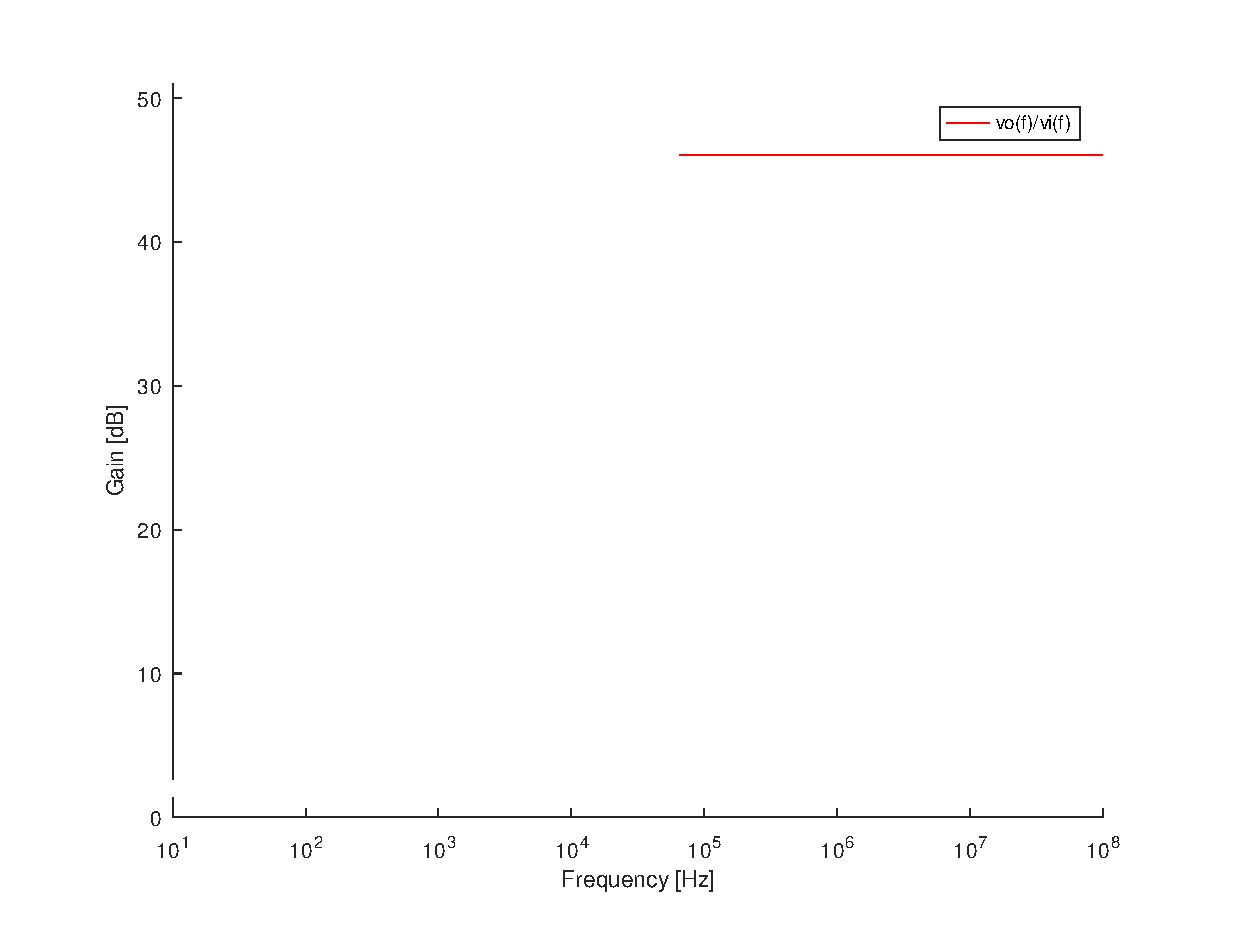
\includegraphics[width=0.6\textwidth]{gain.eps}
	\caption{The voltage gain}
	\label{fig:voltage_gain}
\end{figure}

\paragraph{}Concluding this theoretical analysis of the amplifier, the table below has the voltage gain of the whole circuit, also including its representation in decibels(which is the one used in the graphic above). 

\begin{table}[H]
	\centering
	\begin{tabular}{|l|l|} 
		\hline
		Data             & Values                               \\ 
		\hline
		
Total Voltage Gain     &  -200.038143   \\ \hline
Total Voltage Gain (in dB)   &  46.022256   \\ \hline
	\end{tabular}
\end{table}


